\subsection{正函数的上积分}

对每个定义在 X 上的数值函数 \(f \geqslant 0\) （有限或否），存在函数 \(h \in J_{+}\) 使 \(f \leqslant h\) ，至少还有常值函数 \(+\infty\) 。

定义 3. --- 设 \(\mu\) 是 X 上的正测度；对每个定义在 X 上的数值函数 \(f \geqslant 0\) （有限或否），正数

\[
\mu^ {*} (f) = \inf _ {h \geqslant f, h \in \mathscr {I} _ {+}} \mu^ {*} (h)
\]

（有限或等于 \(+\infty\) ）称为 \(f\) （关于 \(\mu\) ）的上积分。

当 \(f \in \mathcal{I}_+\) 时，这样定义的数 \(\mu^*(f)\) 等于定义 1 中所定义的上积分，因为 \(\mu^*\) 在 \(\mathcal{I}_+\) 上是递增的。

除记号 \(\mu^{*}(f)\) 外，我们还将使用记号 \(\int^{*} f d\mu\) 、\(\int^{*} f(x) d\mu(x)\) 、\(\int^{*} f\mu\) 与 \(\int^{*} f(x)\mu(x)\) 。

例子. --- 若 X 是离散空间，\(\mu\) 是 X 上的一个正测度，且令 \(\alpha(x) = \mu(\varphi_{\{x\}})\) ，则 \(\mu^{*}(f) = \sum_{x \in X} \alpha(x)f(x)\) 对每个数值函数

\(f \geqslant 0\) （定义在 X 上）成立，因为这样的函数是连续的（No.~1, 例子）。

命题 10. --- 若 \(f\) 与 \(g\) 是两个数值函数 \(\geqslant 0\) ，都定义在 \(X\) 上，满足 \(f \leqslant g\) ，则 \(\mu^{*}(f) \leqslant \mu^{*}(g)\) 。

命题 11. --- 对每个有限实数 \(\alpha > 0\) 以及每个定义在 X 上的数值函数 \(f \geqslant 0\) ，

\[
\mu^ {*} (\alpha f) = \alpha \mu^ {*} (f).\tag{8}
\]

命题 12. --- 若 \(f_1\) 与 \(f_2\) 是两个数值函数 \(\geqslant 0\) ，都定义在 \(X\) 上，则

\[
\mu^ {*} (f _ {1} + f _ {2}) \leqslant \mu^ {*} (f _ {1}) + \mu^ {*} (f _ {2}).\tag{9}
\]

对每个函数 \(h_1 \in \mathcal{I}_+\) （满足 \(f_1 \leqslant h_1\) ）以及每个函数 \(h_2 \in \mathcal{I}_+\) （满足 \(f_2 \leqslant h_2\) ），由定理 2 有

\[
\mu^ {*} (f _ {1} + f _ {2}) \leqslant \mu^ {*} (h _ {1} + h _ {2}) = \mu^ {*} (h _ {1}) + \mu^ {*} (h _ {2}),
\]

由此（GT, IV, §5, No.~7, 命题 12 的推论 2）得

\[
\mu^ {*} (f _ {1} + f _ {2}) \leqslant \inf _ {h _ {1} \geqslant f _ {1}, h _ {1} \in \mathcal {I} _ {+}} \mu^ {*} (h _ {1}) + \inf _ {h _ {2} \geqslant f _ {2}, h _ {2} \in \mathcal {I} _ {+}} \mu^ {*} (h _ {2}),
\]

这无非就是不等式 (9)。

命题 10、11 与 12 表明：\(\mu^{*}\) 是定义在 X 上的数值函数 \(\geqslant 0\) 所成之集上的一个递增、正齐次且凸的函数（Ch. I, No.~1）。注意，若 \(f_{1}\) 与 \(f_{2}\) 是任意两个正函数，(9) 的两端不一定相等（ \(\S 4\) ，习题 8 \(d\) ）；在 \(\S 5\) ，No.~6 中我们将给出使等号成立的条件。

定理 3. --- 对每个递增序列 \((f_{n})\) （由定义在 X 上的数值函数 \(\geqslant 0\) 组成），

\[
\mu^ {*} \left(\sup _ {n} f _ {n}\right) = \sup _ {n} \mu^ {*} (f _ {n}).\tag{10}
\]

由于函数 \(f_n\) 每个都小于或等于 \(\sup_{n} f_n\) ，问题归结为证明 \(\mu^*(\sup_{n} f_n) \leqslant \sup_{n} \mu^*(f_n)\) ；若不等式的第二端为 \(+\infty\) ，这是显然的。在相反的情形，\(\mu^*(f_n) < +\infty\) 对一切 \(n\) 成立；我们将证明，对每个 \(\varepsilon > 0\) ，存在递增序列 \((g_n)\) ，其诸函数属于 \(\mathcal{I}_+\) ，满足 \(f_n \leqslant g_n\) 且 \(\mu^*(g_n) \leqslant \mu^*(f_n) + \varepsilon\) 。若 \(g\) 是序列 \((g_n)\) 的上包络，则将有 \(\mu^*(g) = \sup_n \mu^*(g_n)\) （No.~1, 定理 1），由此 \(\mu^*(g) \leqslant \sup \mu^*(f_n) + \varepsilon\) ；由于 \(\sup f_n \leqslant g\) 且 \(\varepsilon\) 任意，定理即得证明。

根据假设，存在函数 \(h_{n} \in I_{+}\) 满足 \(f_{n} \leqslant h_{n}\) 且 \(\mu^{*}(f_{n}) \leqslant \mu^{*}(h_{n}) \leqslant \mu^{*}(f_{n}) + \varepsilon/2^{n}\) ；我们来证明诸函数 \(g_{n} = \sup(h_{1}, h_{2}, \ldots, h_{n})\) 满足要求。它们属于 \(I_{+}\) ，构成一个递增序列，且对所有 n 满足 \(f_{n} \leqslant g_{n}\) ；我们将证明

\[
\mu^ {*} (g _ {n}) \leqslant \mu^ {*} (f _ {n}) + \varepsilon \left(1 - \frac {1}{2 ^ {n}}\right).
\]

对 \(n\) 作归纳论证；情形 \(n = 1\) 是平凡的。另一方面，\(g_{n+1} = \sup(g_n, h_{n+1})\) ，\(g_n \geqslant f_n\) 且 \(h_{n+1} \geqslant f_{n+1} \geqslant f_n\) ，由此 \(\inf(g_n, h_{n+1}) \geqslant f_n\) ；由于

\[
\inf (g _ {n}, h _ {n + 1}) + \sup (g _ {n}, h _ {n + 1}) = g _ {n} + h _ {n + 1},
\]

由 No.~1 的定理 2 推出

\[
\begin{array}{l} \mu^ {*} (g _ {n + 1}) = \mu^ {*} (g _ {n}) + \mu^ {*} (h _ {n + 1}) - \mu^ {*} \big (\inf (g _ {n}, h _ {n + 1}) \big) \\ \leqslant \mu^ {*} (g _ {n}) + \mu^ {*} (h _ {n + 1}) - \mu^ {*} (f _ {n}) \\ \leqslant \mu^ {*} (f _ {n + 1}) + \varepsilon \left(1 - \frac {1}{2 ^ {n}}\right) + \frac {\varepsilon}{2 ^ {n + 1}} \\ = \mu^ {*} (f _ {n + 1}) + \varepsilon \left(1 - \frac {1}{2 ^ {n + 1}}\right). \end{array}\tag{Q.E.D.}
\]

推论. --- 设 F 是数值函数 \(\geqslant 0\) 所成的一个集，按关系 \(\leqslant\) 有向，且存在 F 的一个可数共尾子集 G （S, III, §1, No.~7）；则

\[
\mu^ {*} \left(\sup _ {f \in \mathfrak {F}} f\right) = \sup _ {f \in \mathfrak {F}} \mu^ {*} (f).\tag{11}
\]

事实上，存在 \(\mathfrak{G}\) 中函数的一个递增序列，它与 \(\mathfrak{F}\) 有相同的上包络：若 \((f_n)\) 是 \(\mathfrak{G}\) 的诸函数按任意次序排成的序列，令 \((f_{n_k})\) 为由条件 \(n_1 = 1\) 、\(f_{n_{k+1}} \geqslant \sup(f_{n_k}, f_k)\) 递归地定义的子序列；显然这个子序列具有所指的性质。

\pandocbounded{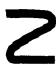
\includegraphics[keepaspectratio]{images/part001_ffa48347.jpg}}

注记. - 1) 当 \(\mathfrak{F}\) 是一个由非下半连续的函数 \(\geqslant 0\) 组成的不可数有向集时，关系式 (11) 不一定成立。例如取 \(X = R\) ，\(\mu\) 为 \(R\) 上的 Lebesgue 测度，并考虑按 \(\leqslant\) 有向的集 \(\mathfrak{F}\) ，它由所有特征函数 \(\varphi_{M}\) （ \(M\) 取遍 \(R\) 的有限子集）组成。这时 \(\mu^{*}(\varphi_{M}) = 0\) 对每个有限子集 \(M\) 成立，因为一点含于一个长度任意小的开区间中，从而由 No.~2 的定义 3 与命题 9，化为一点的集合的特征函数的上积分为零。但 \(\mathfrak{F}\) 的上包络是等于 1 的常值函数，而 \(\mu^{*}(1) = +\infty\) 。

\begin{enumerate}
\def\labelenumi{\arabic{enumi})}
\setcounter{enumi}{1}
\tightlist
\item
  注意，对递减序列 \((f_n)\) （诸函数 \(\geqslant 0\) ），不一定有 \(\mu^{*}(\inf_{n} f_n) = \inf_{n} \mu^{*}(f_n)\) ，即使 \(\mu^{*}(f_n) < +\infty\) 对所有 \(n\) 成立（参见 §4, 习题 8 c)）。
\end{enumerate}

命题 13. --- 对每个序列 \((f_n)\) （诸数值函数 \(\geqslant 0\) ，定义在 \(X\) 上），

\[
\mu^ {*} \left(\sum_ {n = 1} ^ {\infty} f _ {n}\right) \leqslant \sum_ {n = 1} ^ {\infty} \mu^ {*} (f _ {n}).\tag{12}
\]

只需对递增的函数序列 \(g_{n} = \sum_{k=1}^{n} f_{k}\) 应用关系式 (10)，并同时注意到由 (9) 有

\[
\mu^ {*} (g _ {n}) \leqslant \sum_ {k = 1} ^ {n} \mu^ {*} (f _ {k}).
\]

在 §5, No.~6 中，我们将给出使 (12) 的两端相等的条件。

命题 14（Fatou 引理）. --- 对每个序列 \((f_{n})\) （诸数值函数 \(\geqslant 0\) ），

\[
\mu^ {*} \left(\liminf _ {n \to \infty} f _ {n}\right) \leqslant \liminf _ {n \to \infty} \mu^ {*} (f _ {n})  .\tag{13}
\]

对每个整数 \(n\) ，令 \(g_{n} = \inf_{p\geqslant 0}f_{n + p}\) ；序列 \((g_n)\) 递增，且 \(\liminf_{n\to \infty}f_n = \sup_n g_n\) ，由此，由 (10) 得

\[
\mu^ {*} (\liminf _ {n \to \infty} f _ {n}) = \sup _ {n} \mu^ {*} (g _ {n});
\]

但由于 \(g_{n} \leqslant f_{n+p}\) 对 \(p \geqslant 0\) 成立，有 \(\mu^{*}(g_{n}) \leqslant \mu^{*}(f_{n+p})\) ，由此 \(\mu^{*}(g_{n}) \leqslant \inf_{p \geqslant 0} \mu^{*}(f_{n+p})\) ，最终得

\[
\mu^ {*} \left(\operatorname * {l i m i n f} _ {n \to \infty} f _ {n}\right) \leqslant \sup _ {n} \left(\inf _ {p \geqslant 0} \mu^ {*} (f _ {n + p})\right) = \operatorname * {l i m i n f} _ {n \to \infty} \mu^ {*} (f _ {n}).
\]

推论. --- 设 \((f_{n})\) 是数值函数 \(\geqslant0\) 的一个序列，使得对每个 \(x\in X\) ，\(\lim_{n\to\infty}f_{n}(x)=+\infty\) 。若 \(\mu\) 不是零测度，则 \(\lim_{n\to\infty}\mu^{*}(f_{n})=+\infty\) 。

若 \(f_{0}\) 是等于 \(+\infty\) 的常值函数，则 \(f_{0}\) 是 \(K_{+}\) 中所有函数的上包络，且由于 \(\mu \neq 0\) ，有 \(\mu^{*}(f_{0}) > 0\) ；但由于 \(f_{0} = \alpha f_{0}\) 对每个 \(\alpha > 0\) 成立，必然有 \(\mu^{*}(f_{0}) = +\infty\) （命题 11）。于是不等式 (13) 表明 \(\mu^{*}(f_{n})\) 随 n 趋于 \(+\infty\) 。

命题 15. --- 对每个标量 \(\alpha > 0\) 以及每一对正测度 \(\mu, \nu\) （在 \(X\) 上），

\[
(\alpha \mu) ^ {*} = \alpha \mu^ {*}\tag{14}
\]

\[
(\mu + \nu) ^ {*} = \mu^ {*} + \nu^ {*}\tag{15}
\]

此外，关系 \(\mu \leqslant \nu\) 蕴含 \(\mu^{*} \leqslant \nu^{*}\) 。

我们来证明关系式 (15)。令 \(\lambda = \mu + \nu\) ；于是 \(\lambda(f) = \mu(f) + \nu(f)\) 对 \(f \in \mathcal{K}_+\) 成立；对 \(f \in \mathcal{I}_+\) ，\(\lambda^*(f)\) （相应地 \(\mu^*(f), \nu^*(f)\) ）的值是 \(\lambda(g)\) （相应地 \(\mu(g), \nu(g)\) ）当 \(g\) 跑遍（按 \(\leqslant\) 有向的）所有 \(g \in \mathcal{K}_+\) （满足 \(g \leqslant f\) ）所成之集时的极限；因此 \(\lambda^*(f) = \mu^*(f) + \nu^*(f)\) 。最后，若 \(f\) 是定义在 X 上的任一函数 \(\geqslant 0\) ，则 \(\lambda^*(f)\) （相应地 \(\mu^*(f), \nu^*(f)\) ）是 \(\lambda^*(h)\) （相应地 \(\mu^*(h), \nu^*(h)\) ）当 \(h\) 跑遍（按 \(\geqslant\) 有向的）所有函数 \(h \in \mathcal{I}_+\) （满足 \(h \geqslant f\) ）所成之集时的极限；再次取极限，便得 \(\lambda^*(f) = \mu^*(f) + \nu^*(f)\) ，这就证明了 (15)。关系式 (14) 类似地建立。最后，若 \(\mu \leqslant \nu\) ，则可写 \(\nu = \mu + (\nu - \mu)\) ，其中 \(\nu - \mu \geqslant 0\) ，因此 \(\nu^* = \mu^* + (\nu - \mu)^*\) ，这表明 \(\mu^* \leqslant \nu^*\) 。

